
\iffalse 
Assignment 4
Date    : 12th March 2021
Course  : Applied Programming Lab(EE2703)
Faculty : Prof. Harishankar Ramachandhran

Submission by : Santosh G (EE19B055)

To complie and get the Report(PDF):
1) python3 EE2703_ASSIGN4_EE19B055.py  (Atleast Once, for the plots)
2) pdflatex EE2703_ASSIGN4_EE19B055.tex
 
PS: Run "EE2703_ASSIGN4_EE19B055.py" using the above command atleast once before running this code, as this program needs the plots.
\fi
\documentclass[11pt, a4paper]{article}
\usepackage{graphicx}
\usepackage{amsmath}
\usepackage[margin=0.6in]{geometry}
\usepackage{listings}
\usepackage{float}

\title{APL(EE2703): Assignment 4} % Title
\author{Santosh G  (EE19B055)} % Author name
\date{\today} % Date for the report

\begin{document}
    \maketitle % Insert the title, author and date

    \section{Aim of the Assignment:}
        \begin{itemize}
            \item To find the Fourier coefficients of the given functions: $e^x$ and $cos(cos(x))$
            \item Analyze few of the properties and approximations of the coeeficients.
        \end{itemize}
        This shall be achieved by using two methods: Direct Integration and Least Squares Method, which shall also be compared to the true function.
    \section{Introduction}
    From the Fourier series concept, we know that any periodic function $f(x)$ can be expressed as follows
        
        \begin{equation}
            f(x) = a_0 + \sum_{k=1}^{\infty}a_kcos(kx) + b_ksin(kx)
        \end{equation}
        \\
        \\where $a_0$, $a_k$ and $b_k$ are known as the fourier coefficients.\\
        \\The same can be done with non-periodic functions by taking extensions.\\
        \\These coefficients shall be found out using \textbf{Direct Integragtion} and the \textbf{Least Squares} Methods. 
         
         
	\section{Questions}
	   \subsection{Question 1}
           The function $cos(cos(x))$ is periodic with a fundamental period of ${2\pi}$, whereas $e^x$ is not periodic, rather is a monotonically increasing function.\\
           \\As the period of $cos(cos(x))$ is ${2\pi}$ and we are calculating fourier coffeicints from the interval of same length, we cover all the coefficients and when the function is rebuilt using those coefficients, the actual function is retrieved, without any distortion.\\
           In case of $e^x$ the function calculated will be shifted version of function that exist in the [0, ${2\pi}$]. \\
           \\
           The above statements have been clearly depicted in the following figures:            
            \begin{figure}[H]
                \centering
                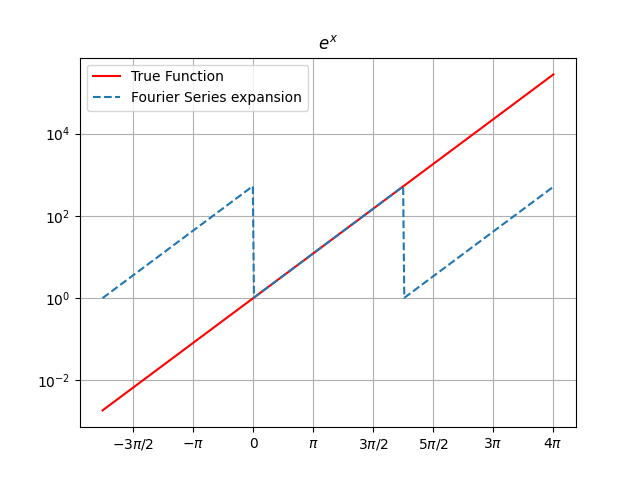
\includegraphics[scale=0.9]{Figure 1.png}
                \caption{Actual function vs Generated function for $e^x$ (Plot for Q1)}              
            \end{figure}
            
            \begin{figure}[H]
                \centering
                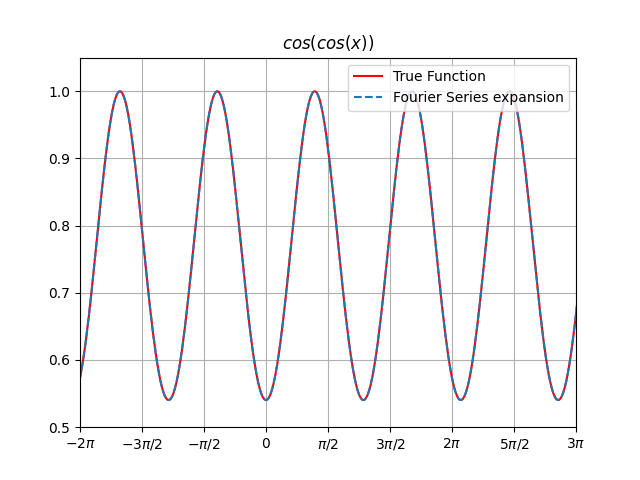
\includegraphics[scale=0.9]{Figure 2.png}
                \caption{Actual function vs Generated function for $cos(cos(x))$ (Plot for Q1)}    
            \end{figure}
       
	  \subsection{Question 3}
	  a) We know that $cos(cos(x))$ is an even function and calculation of $b_n$ will lead to integration of an odd integrand giving zero as the final output.\\
	  PS: There is negligible error due to approximations of function \textit{"quad"}.\\
	  \\b) In case of \textit{exp(x)}, sinusoids of higher frequency are also required to approximate the series due to the monotonicity(no oscillation), whereas in the case of \textit{cos(cos(x))}, the frequency is limited and hence lower order terms are sufficient to get a good fit, hence the decay of coefficients is much faster in the second case(i.e $cos(cos(x))$).\\
	  \\c) The coefficients $a_n$ and $b_n$ of $exp(x)$ are proportional to the following and the assumptions can be made as shown:\\
          \\  \begin{equation}
                 a_n \propto \frac{1}{n^2 + 1} , b_n \propto \frac{n}{n^2 + 1}
            \end{equation}
            For sufficiently large n
            \begin{equation}
                 a_n \approx \frac{1}{n^2},  b_n \approx \frac{1}{n}
            \end{equation}		
	    \\
	    \begin{equation}
                 log(a_n) \approx -2log(n),  b_n \approx -log(n)
            \end{equation}		
	 \\
	 Hence as shown above, the LogLog plots of $exp(x)$ is linear.\\
	    \\Simlarly, the coefficients of $cos(cos(x))$ vary in exponential orders of "n" and hence the semilog plt is linear.
        \\
        \\
             Plots for the above are given Below:
            \begin{figure}[H]
                    \centering
                    \setlength\tabcolsep{2pt}
                    \begin{tabular}{cc}
                       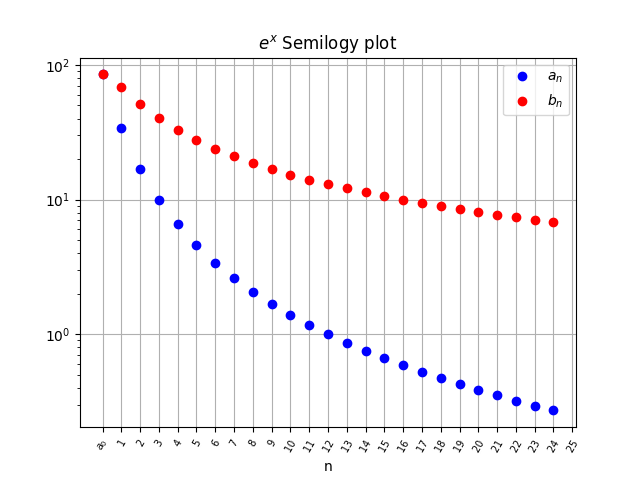
\includegraphics[scale=0.5]{Figure 3.png} &
                       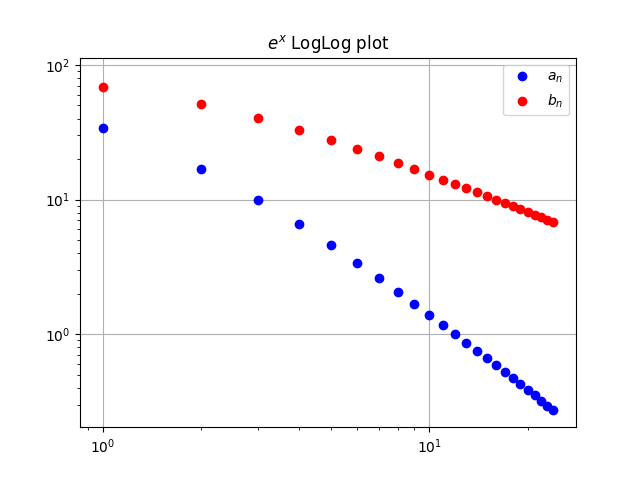
\includegraphics[scale=0.5]{Figure 4.png}
                    \end{tabular}
                    \caption{Semilog Plot of $exp(x)$ (Left)} \caption{Loglog plot of $exp(x)$ (Right)}
                \end{figure}
                
             \begin{figure}[H]
                    \centering
                    \setlength\tabcolsep{2pt}
                    \begin{tabular}{cc}
                       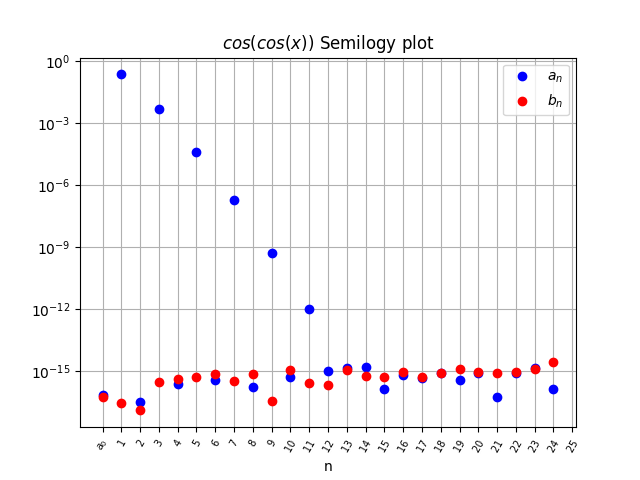
\includegraphics[scale=0.5]{Figure 5.png} &
                       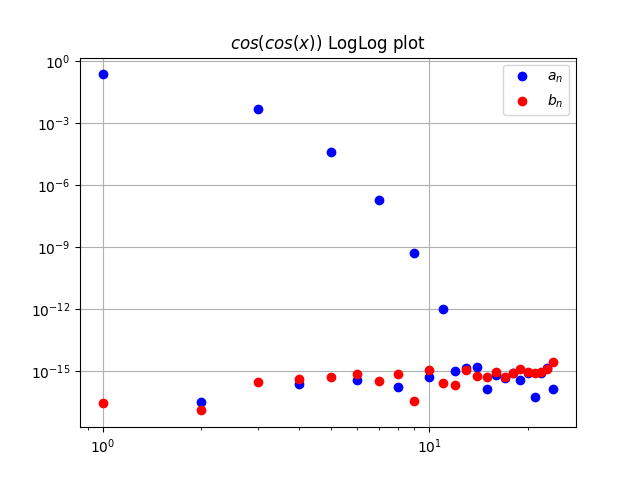
\includegraphics[scale=0.5]{Figure 6.png}
                    \end{tabular}
                    \caption{Semilog Plot of $cos(cos(x))$ (Left)} \caption{Loglog plot of $cos(cos(x))$ (Right)}
                \end{figure}
                
	   \subsection{Question 5}
           Best fit of the coefficients of the functions $cos(cos(x))$ ans $exp(x)$ have been calculated and Plotted in the figures 11 and 12, following.            

            
            \subsection{Question 6}
           The coefficients of the functions $cos(cos(x))$ ans $exp(x)$ have been calculated through two different methods and the same are being compared in the following plots:
             \begin{figure}[H]
                    \centering
                    \setlength\tabcolsep{2pt}
                    \begin{tabular}{cc}
                       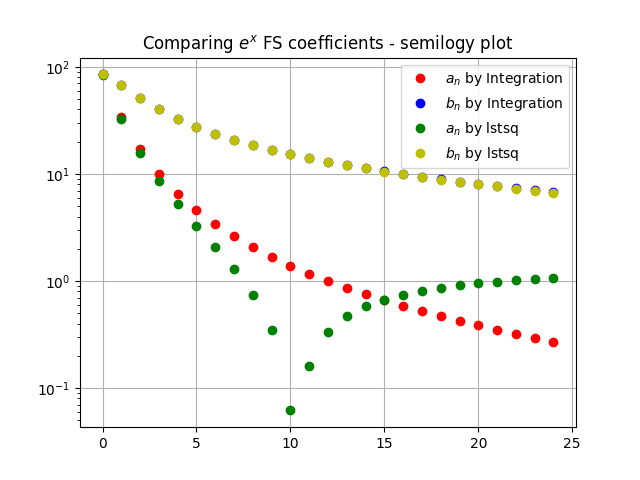
\includegraphics[scale=0.5]{Figure 3.1.png} &
                       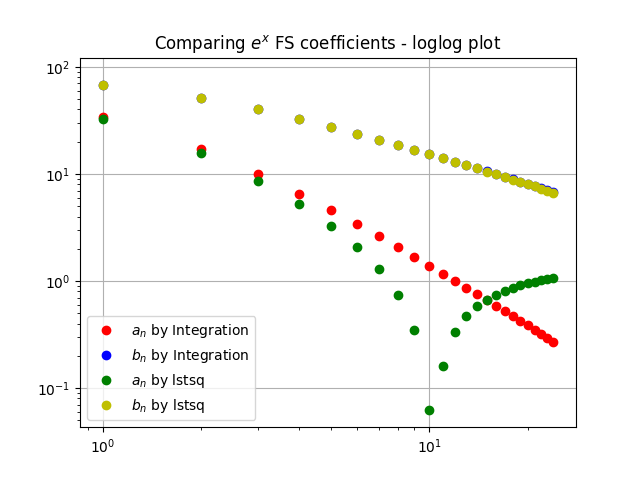
\includegraphics[scale=0.5]{Figure 4.1.png}
                    \end{tabular}
                    \caption{Comaprision of coefficients of $exp(x)$ using a SemiLog plot (Left)}
                    \caption{Comaprision of coefficients of $exp(x)$ using a LogLog plot (Right)}
                \end{figure}
                
             \begin{figure}[H]
                    \centering
                    \setlength\tabcolsep{2pt}
                    \begin{tabular}{cc}
                       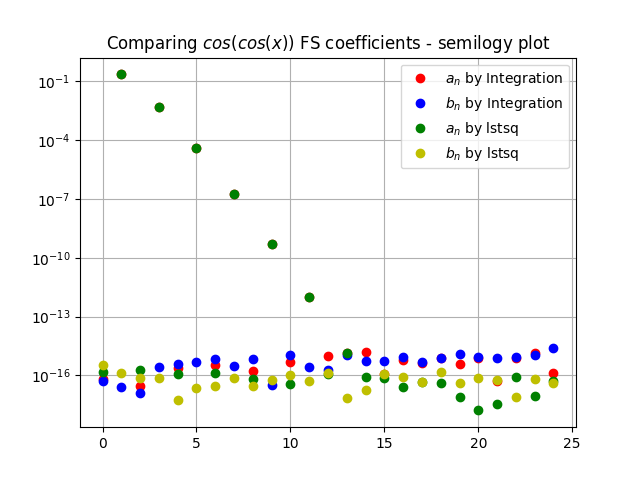
\includegraphics[scale=0.5]{Figure 5.1.png} &
                       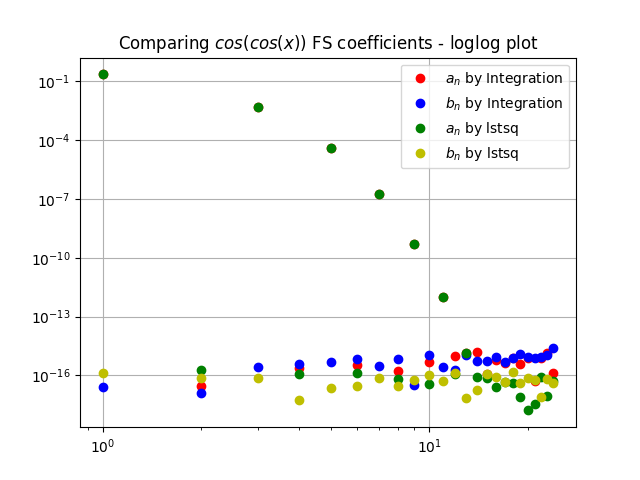
\includegraphics[scale=0.5]{Figure 6.1.png}
                    \end{tabular}
                     \caption{Comaprision of coefficients of $cos(cos(x))$ using a SemiLog plot (Left)}
                     \caption{Comaprision of coefficients of $cos(cos(x))$ using a LogLog plot (Right)}
                    \end{figure}        
    
           The error between the coefficients have been calculated and the results are as following.
           
            \begin{verbatim}
             Maximum deviation for cos(cos(x)) : 2.637612449475514e^-15
             Maximum deviation for exp(x)      : 1.332730870335368
            \end{verbatim}
            
           \subsection{Question 7}
           In case $exp(x)$ the coefficients calculated in different ways do not agree with because of the fact that $exp(x)$ is non periodic and we have considered only 51 coefficients, the higher frequencies also play a crucial role.
           \\In case of $cos(cos(x))$ the coefficients are almost the same irrespective of the method, used to calculate.
           \\ The same is evident from the following figures 11 and 12.            
            \begin{figure}[H]
                \centering
                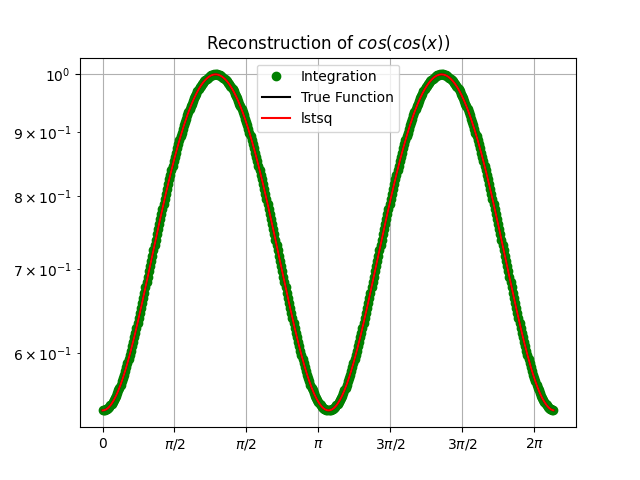
\includegraphics[scale=0.9]{Figure 7.png}
                \caption{Calculated and actual Coefficients for $exp(x)$}                
            \end{figure}                
            \begin{figure}[H]
                \centering
                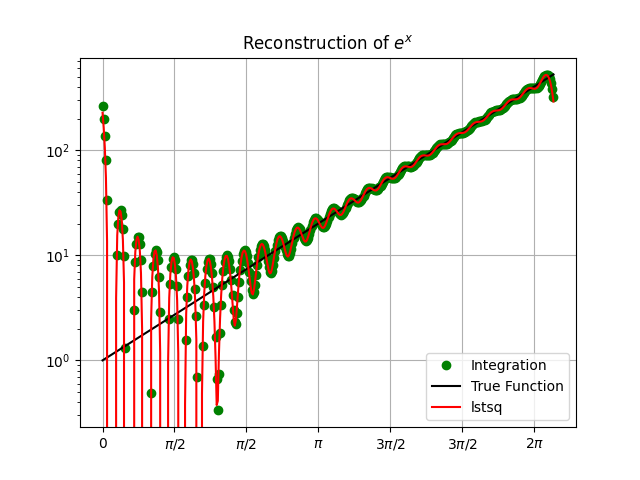
\includegraphics[scale=0.9]{Figure 8.png}
                \caption{Calculated and actual Coefficients for $exp(x)$}                
            \end{figure}
                     
    \section{Conclusion}
      The fourier co-efficients of both the functions ${cos(cos(x))}$ and ${exp(x)}$ have been calculated through two different methods, "Least Squares" and "Integration" and using least squares has given a better results.\\
      \\The coefficients of $cos(cos(x))$ match perfectly with true value as the sample is considered in the interval equal to its periodicity, whereas we can observe mismatches in case of $exp(x)$ at boundaries(i.e 0 and 2pi), due to the discontinuities of the actual function and the periodic extensions.\\
     \\
      The fourier series coefficients can be approximated with near perfection if the function is periodic and there are no discontinuities either in the interval or at the boundaries. These discontinuites would result in distortions and errors in Fourier coefficients as observed in case of $exp(x)$
\end{document}
